\documentclass{article}

\usepackage[german]{babel}
\usepackage{array}
\usepackage[letterpaper,top=2cm,bottom=2cm,left=3cm,right=3cm,marginparwidth=1.75cm]{geometry}

\usepackage{amsmath}
\usepackage{graphicx}
\usepackage{subcaption} % Added package
\usepackage[colorlinks=true, allcolors=blue]{hyperref}
\usepackage[T1]{fontenc}
\usepackage{tabularx}
\usepackage{booktabs}


\title{Übungsprotokoll - NWG2 - Übung 7 \\ Grande Finale}
\author{\vspace{0.5cm} Thomas Brandstetter (s2210239002) \& Jakob Mayr (s2210239021)}

\begin{document}
\maketitle

\section{Konfiguration der Endsysteme}

In der folgenden Übung haben wir die PCs 4.1 und 4.2 benutzt, somit sind die Netze 4.x verwendet worden. Die IP-Konfiguration wird folgendermaßen vergeben: Klick auf „Network“ in der Taskleiste $\rightarrow$ „Network \& Internet Settings“ $\rightarrow$ „Change adapter options“ $\rightarrow$ gewünschtes Netzwerk Interface auswählen, in diesem Fall Ethernet 2 $\rightarrow$ „Properties“ $\rightarrow$ Doppelklick auf „Internet Protocol Version 4“ bzw. „Internet Protocol Version 6“. In den geöffneten Fenstern können wir nun jeweils die IP-Adresse, Subnetzmaske/Präfix und das Gateway eingeben. Folglich sind die Konfigurationen beider PCs zu sehen:

\begin{figure}[!htp]
  \centering
  \begin{minipage}[b]{0.45\textwidth}
    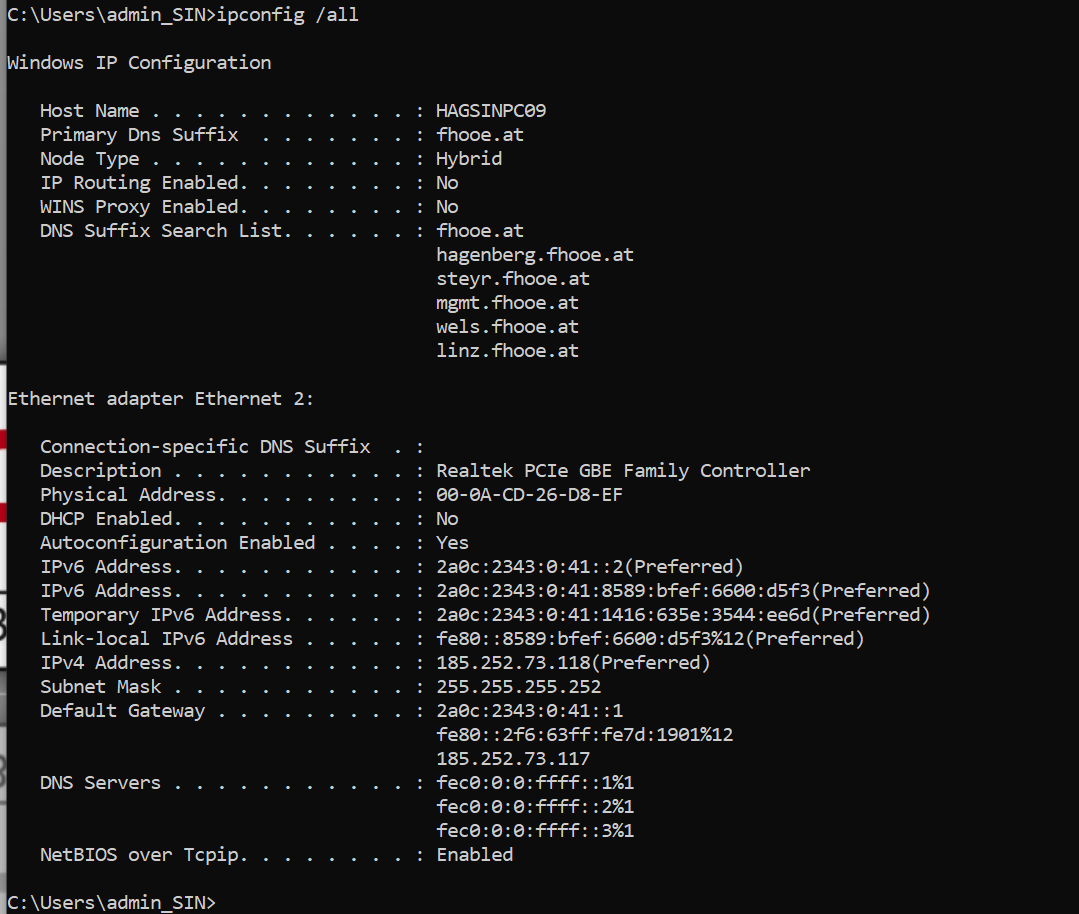
\includegraphics[width=\textwidth]{Arbeitsergebnisse/pc41/pc41_ipconfig.PNG}
    \caption{PC41 IPv4 und IPv6 config}
  \end{minipage}
  \hspace{0.8cm}
  \begin{minipage}[b]{0.45\textwidth}
    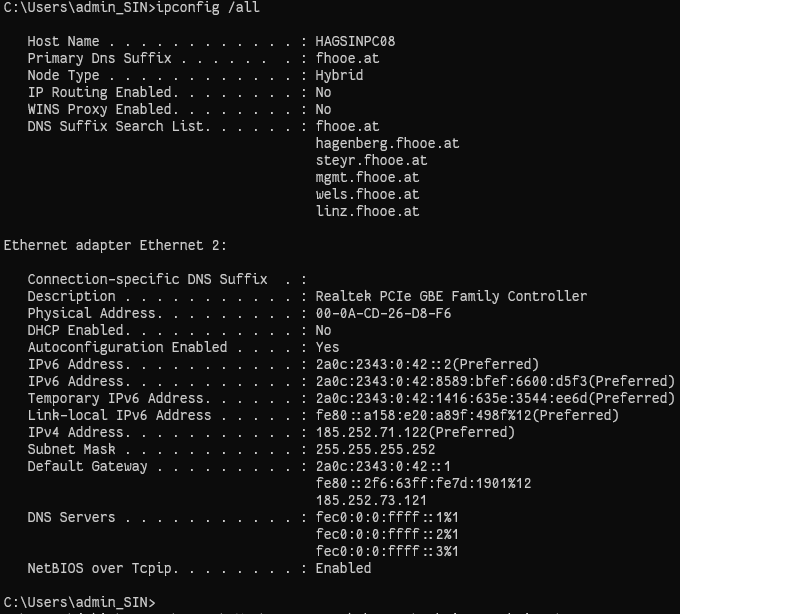
\includegraphics[width=\textwidth]{Arbeitsergebnisse/pc42/pc42_ipconfig.PNG}
    \caption{PC42 IPv4 und IPv6 config}
  \end{minipage}
\end{figure}

\pagebreak



\section{Konfiguration der Gruppenswitches GS41 \& GS42 \& ToR}

\subsection{Konfigurieren der VLANs}

Auf dem unteren Switch (GS41) sollen die VLANS 110 und 120 angelegt werden.\\
Die Ports mit den PCs sollen als Access Port konfiguriert werden: der linke PC (PC41) soll im VLAN 110 sein, und der rechte PC (PC42) im VLAN 120.\\
Der Port zum Router soll als Trunk Port konfiguriert werden, und die VLANs 110 und 120 erlaubt werden. \\
\\
Auf dem oberen Switches (GS42, ToR) soll nur das VLAN 190 angelegt werden.\\
Alle angeschlossenen Ports sollen als Trunk Port konfiguriert werden, und nur das VLAN 190 erlaubt werden\\

\begin{table}[htbp]
    \centering
    \begin{tabularx}{\textwidth}{|X|X|}
        \toprule
        \textbf{Befehl} & \textbf{Erklärung} \\
        \midrule
        switchport access vlan <vlan-tag-numbers> & Mit diesem Befehl wird ein Switchport im „access mode“ einem oder mehreren VLANS zugeordnet.\\
        \hline
        switchport mode access & Mit diesem Befehl wird ein switchport in den „access mode“ gesetzt.\\
        \hline
        switchport mode trunk & Mit diesem Befehl wird ein switchport in den „trunk mode“ gesetzt.\\
        \hline
         switchport trunk allowed vlan <vlan-tag-numbers> & Mit diesem Befehl wird ein switchport im „trunk mode“ einem oder mehreren VLANS zugeordnet.\\
        \bottomrule
    \end{tabularx}
    \caption{Verwendete Befehle zur Konfiguration der Switches}
\end{table}


\section{Konfiguration der Gruppenrouter GR41 \& GR42}

\subsection{Interfaces}
Auf den Routern sind den VLANs entsprechende Subinterfaces anzulegen\\
Auf dem unteren Router (GR41) sollen Subinterfaces zu allen anliegenden VLANs (110, 120, bzw. 190) angelegt werden.\\
Auf dem oberen Router (GR42) sollen Subinterfaces zum VLAN 190 angelegt werden.\\

\begin{table}[htbp]
    \centering
    \begin{tabularx}{\textwidth}{|X|X|}
        \toprule
        \textbf{Befehl} & \textbf{Erklärung} \\
        \midrule
        encapsulation dot1Q <vlan-tag-number> & Mit diesem Befehl wird ein Interface einem VLAN zugewiesen.\\
        \hline
        ip address <ip-address> <ip-address-mask> & Mit diesem Befehl wird einem dem ausgewählten Interface eine IPv4-Adresse und Maske zugewiesen.\\
        \hline
        ipv6 address <ip-address/ip-address-mask> & Mit diesem Befehl wird einem dem ausgewählten Interface eine IPv6-Adresse und Maske zugewiesen.\\
        \bottomrule
    \end{tabularx}
    \caption{Verwendete Befehle zur Konfiguration der Gruppenrouter}
    \label{tab:commands}
\end{table}

\pagebreak

\subsection{Routen}
Dynamische Routen sollen mit OSPF für IPv4 und IPv6 konfiguriert werden.\\
Für alle Netze bzw. Interfaces des unteren Routers.\\
Für das dem Netz 4.0 des oberen Routers bzw. demjenigen Interface, dem
dieses Netz angehört.\\
\\
Statische Routen sollen für IPv4 und IPv6 manuell konfiguriert werden.\\
Default Routen für den unteren Router.\\
Summary Routen zu allen anderen Gruppen.\\

\begin{table}[htbp]
    \centering
    \begin{tabularx}{\textwidth}{|X|X|}
        \toprule
        \textbf{Befehl} & \textbf{Erklärung} \\
        \midrule
        ipv6 unicast-routing & Dieser Befehl aktiviert "unicast-routing".\\
        ip <routenetwork-number> <network-mask> <ip-address> | interface> & Mit diesem Befehl wird eine statische IPv4 Route in der Routing-Tabelle angelegt.\\
        \hline
        ipv6 <routenetwork-number/network-mask> <ip-address | interface> & Mit diesem Befehl wird eine statische IPv6 Route in der Routing-Tabelle angelegt.\\
        \hline
        router ospf <number> & Legt Router für IPv4 an.\\
        \hline
        network <address> <inverted subnetmask> area <area-number> & Verbindet ein Netzwerk mit einem "RIP" (Routing Prozess).\\
        \hline
        ipv6 ospf1 area <area-number> & Legt Router für IPv6 an.\\
        \bottomrule
    \end{tabularx}
    \caption{Verwendete Befehle zur Konfiguration der Gruppenrouter}
    \label{tab:commands}
\end{table}


\section{Konfiguration der Per VLAN Spanning Trees (PVST)}
Da während der Übung die Gruppen unterschiedlich schnell fertig wurden und Gruppe 5 ihre Verbindungen bereits abgebaut hat, konnte der spanning-tree von unserer Seite her leider nicht mehr demonstiert werden.\\
Im folgenden ist jedoch der Spanning-Tree aus sicht von Gruppe 5 zu sehen. Klar zu erkennen ist, dass die Verbindungen auf Interface Gi1/0/2 und Gi1/0/3 im Status "block"/"BLK" sind.

\begin{figure}[!htp]
  \centering
  \begin{minipage}[b]{0.90\textwidth}
    \includegraphics[width=\textwidth]{Arbeitsergebnisse/gs52/gs52_span.jpeg}
    \caption{GS52 show spanning-tree}
  \end{minipage}
\end{figure}

\pagebreak
\section{Tests und Interpretation ihrer Resultate}

\subsection{PC41 \& PC42}
Pings von PC41 zu PC42, PC81 und PC82.\\
\begin{figure}[!htp]
  \centering
  \begin{minipage}[b]{0.25\textwidth}
    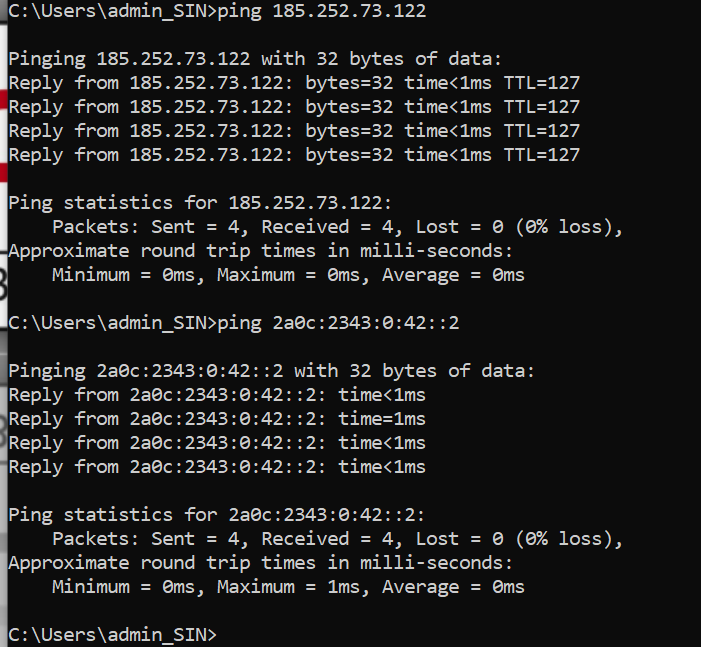
\includegraphics[width=\textwidth]{Arbeitsergebnisse/pc41/pc41_ping_pc42.PNG}
    \caption{PC41 ping PC42}
  \end{minipage}
  \hspace{0.8cm}
  \begin{minipage}[b]{0.25\textwidth}
    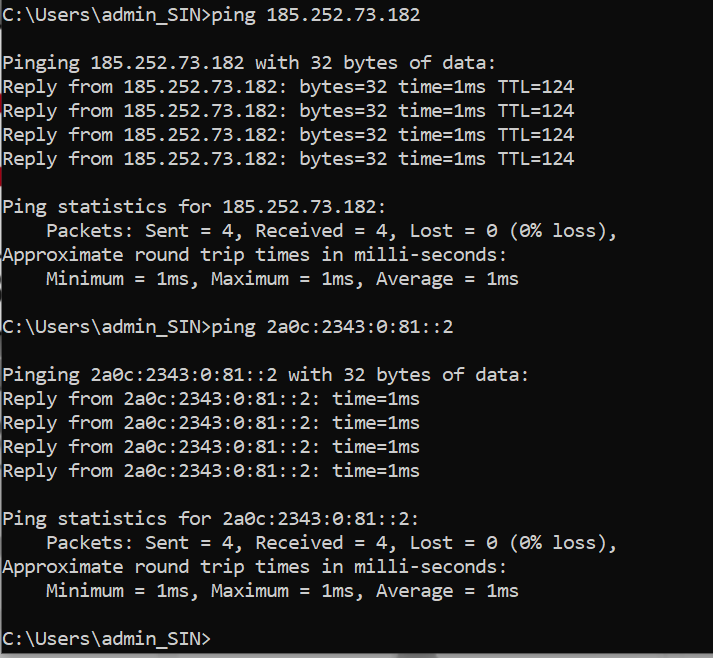
\includegraphics[width=\textwidth]{Arbeitsergebnisse/pc41/pc41_ping_pc81.PNG}
    \caption{PC41 ping PC81}
  \end{minipage}
  \hspace{0.8cm}
  \begin{minipage}[b]{0.25\textwidth}
    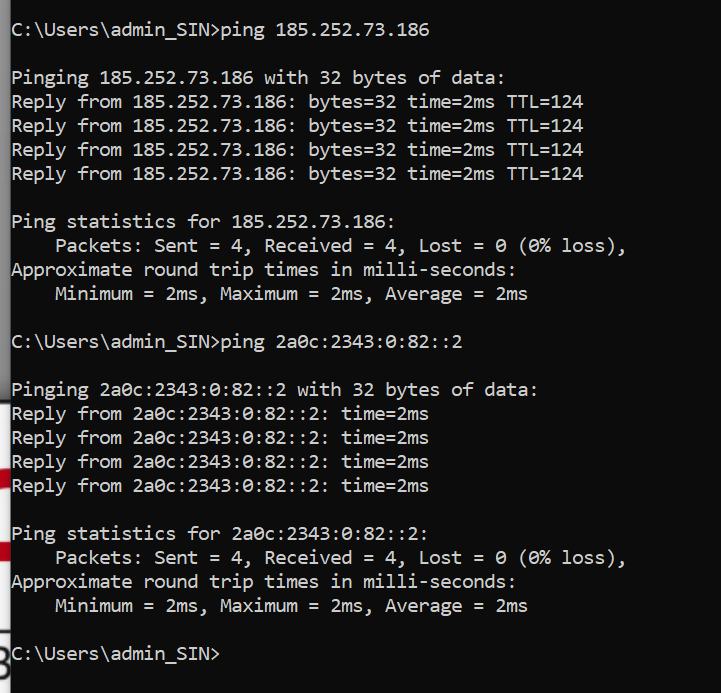
\includegraphics[width=\textwidth]{Arbeitsergebnisse/pc41/pc41_ping_pc82.PNG}
    \caption{PC41 ping PC82}
  \end{minipage}
\end{figure}

Pings von PC42 zu PC41, PC81 und PC82.\\
\begin{figure}[!htp]
  \centering
  \begin{minipage}[b]{0.25\textwidth}
    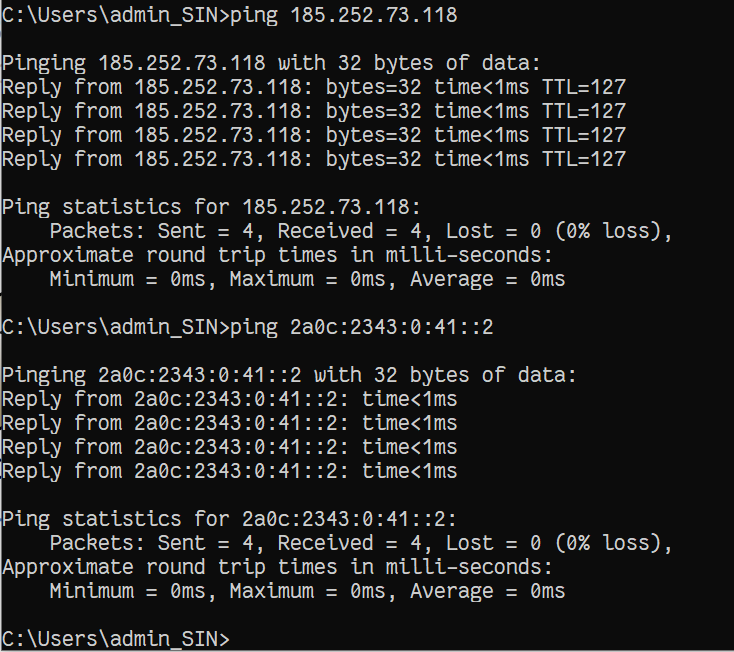
\includegraphics[width=\textwidth]{Arbeitsergebnisse/pc42/pc42_ping_pc41.PNG}
    \caption{PC42 ping PC41}
  \end{minipage}
  \hspace{0.8cm}
  \begin{minipage}[b]{0.25\textwidth}
    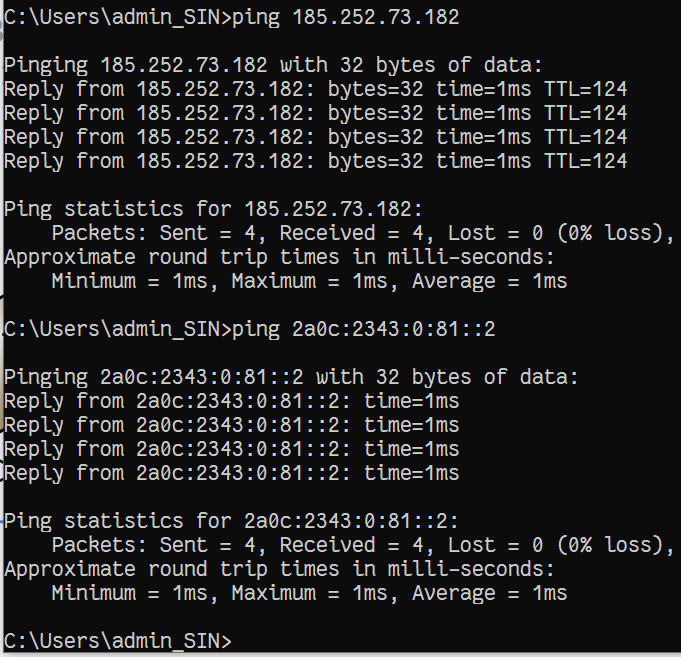
\includegraphics[width=\textwidth]{Arbeitsergebnisse/pc42/pc42_ping_pc81.PNG}
    \caption{PC42 ping PC81}
  \end{minipage}
  \hspace{0.8cm}
  \begin{minipage}[b]{0.25\textwidth}
    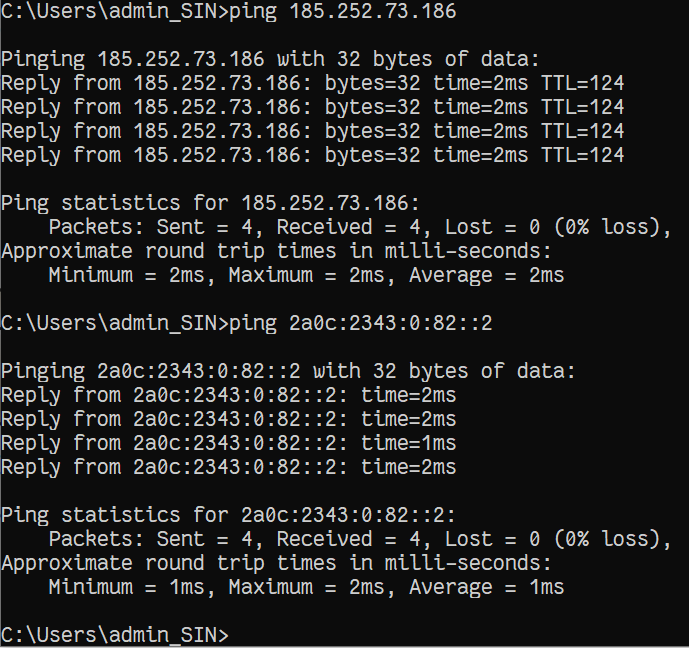
\includegraphics[width=\textwidth]{Arbeitsergebnisse/pc42/pc42_ping_pc82.PNG}
    \caption{PC42 ping PC82}
  \end{minipage}
\end{figure}

\pagebreak

\subsection{GS42}
Folglich ist der spanning-tree des Gruppenswitches GS42 zu sehen. Da wie bereits erwähnt Gruppe 5 bereits fertig abgebaut hat, sind in dieser Grafik keine geblockten Interfaces zu sehen.\\
\begin{figure}[!htp]
  \centering
  \begin{minipage}[b]{0.90\textwidth}
    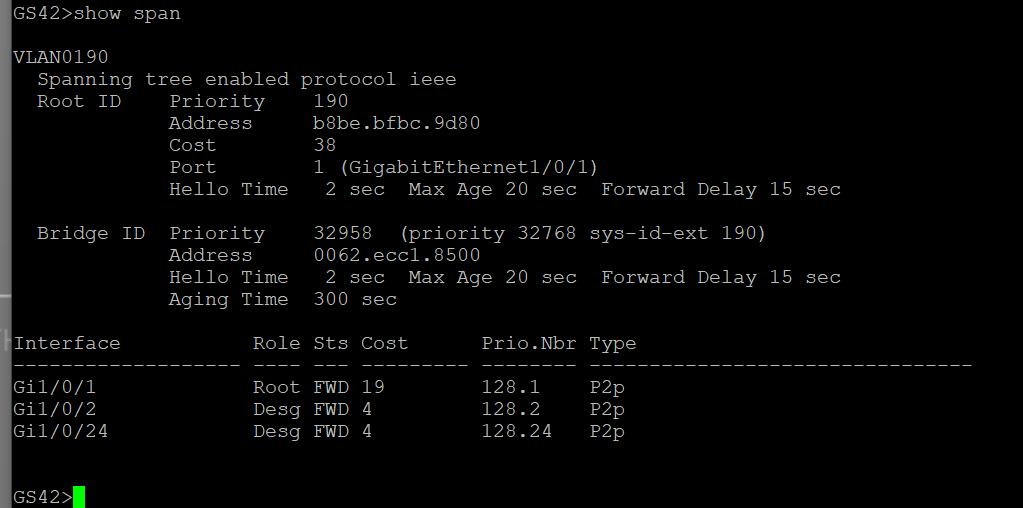
\includegraphics[width=\textwidth]{Arbeitsergebnisse/gs42/gs42_span.png}
    \caption{GS42 show spanning-tree}
  \end{minipage}
\end{figure}


\subsection{GR41}
Folglich sind die Routen (IPv4 \& IPv6) von GR41 und ein ping zu GR42 zu sehen. Die Routen zeigen die direkt verbundenen Geräte, die statisch Konfigurierten Routen, wie auch die durch OSPF vom GS42 gelernten Routen.\\
\begin{figure}[!htp]
  \centering
  \begin{minipage}[b]{0.45\textwidth}
    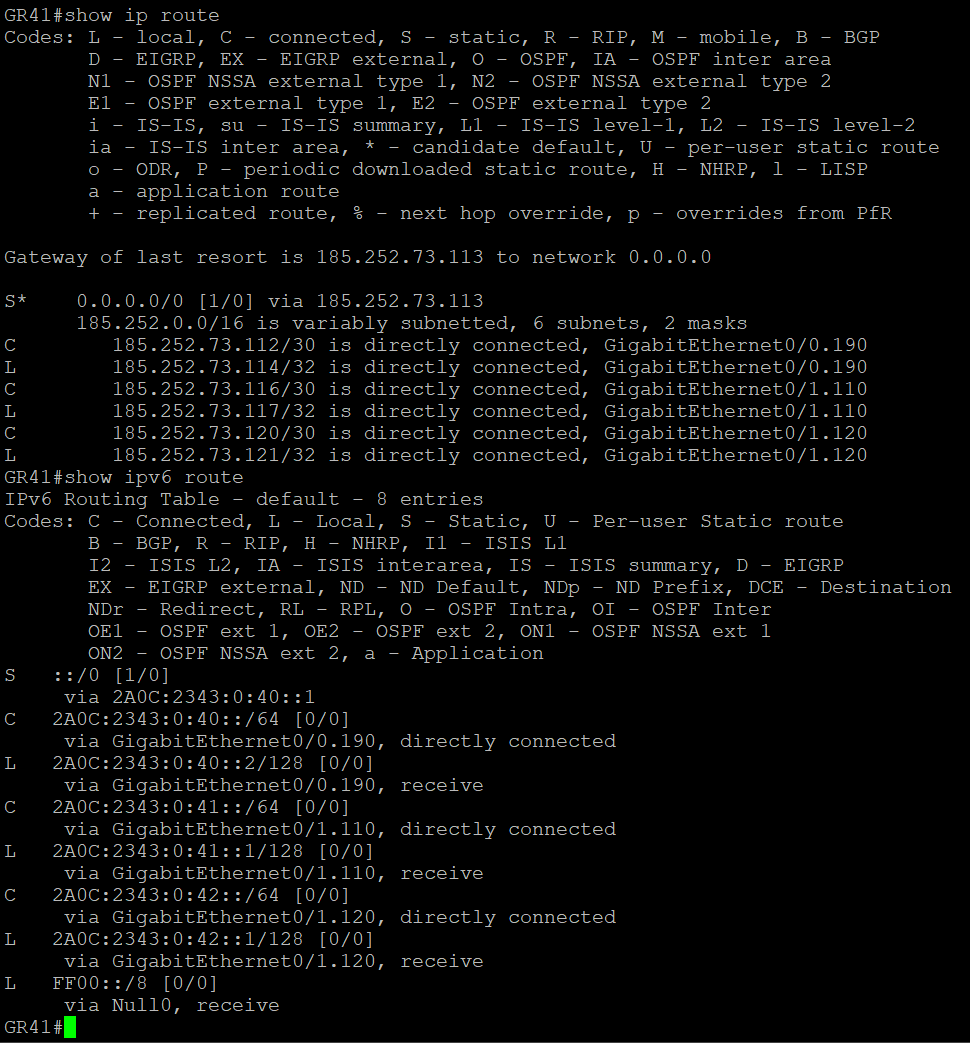
\includegraphics[width=\textwidth]{Arbeitsergebnisse/gr41/gr41_show_route.png}
    \caption{GR41 show route (IPv4 \& IPv6)}
  \end{minipage}
  \hspace{0.8cm}
  \begin{minipage}[b]{0.45\textwidth}
    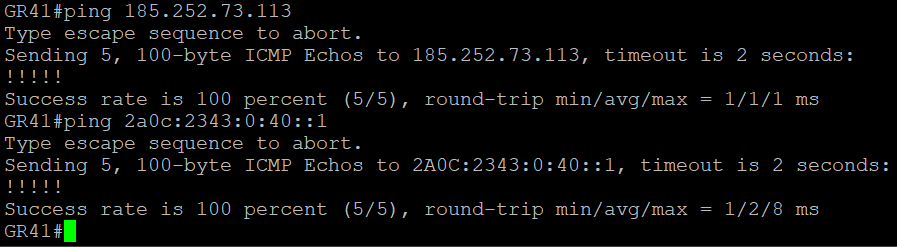
\includegraphics[width=\textwidth]{Arbeitsergebnisse/gr41/gr41_ping_gr42.PNG}
    \caption{GR42 ping GR42}
  \end{minipage}
\end{figure}

\subsection{GR42}
Folglich sind die Routen (IPv4 \& IPv6) von GR42 zu sehen. Die Routen zeigen die direkt verbundenen Geräte, die statisch Konfigurierten Routen, wie auch die OSPF Routen.\\
\begin{figure}[!htp]
  \centering
  \begin{minipage}[b]{0.45\textwidth}
    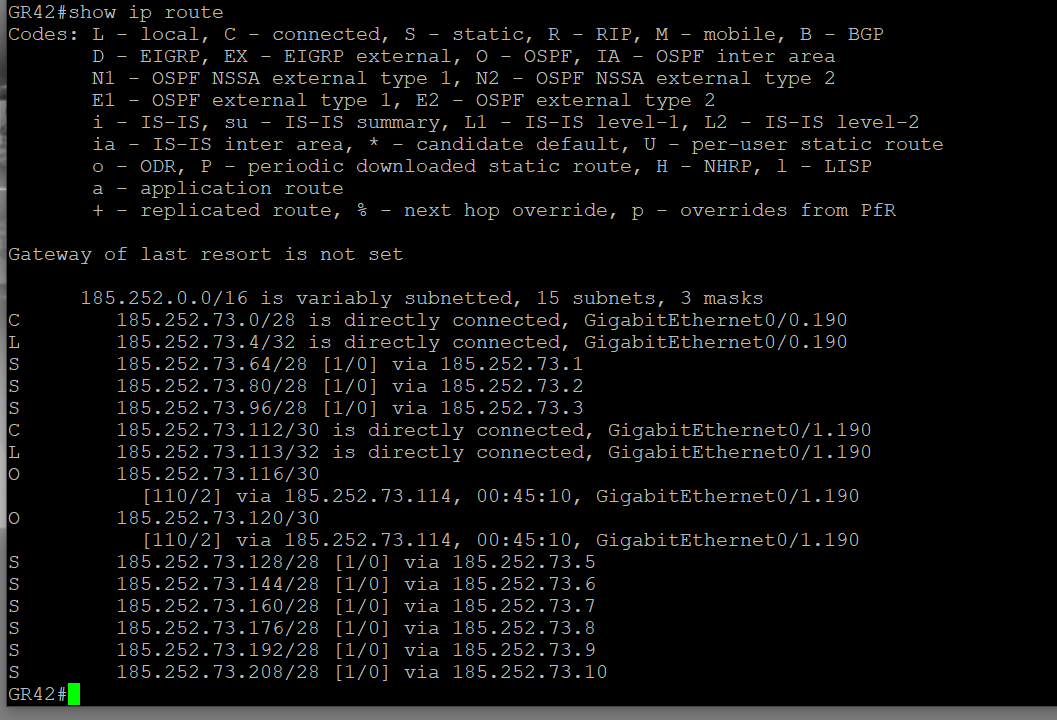
\includegraphics[width=\textwidth]{Arbeitsergebnisse/gr42/gr42_show_ip_route.png}
    \caption{GR42 show route (IPv4)}
  \end{minipage}
  \hspace{0.8cm}
  \begin{minipage}[b]{0.45\textwidth}
    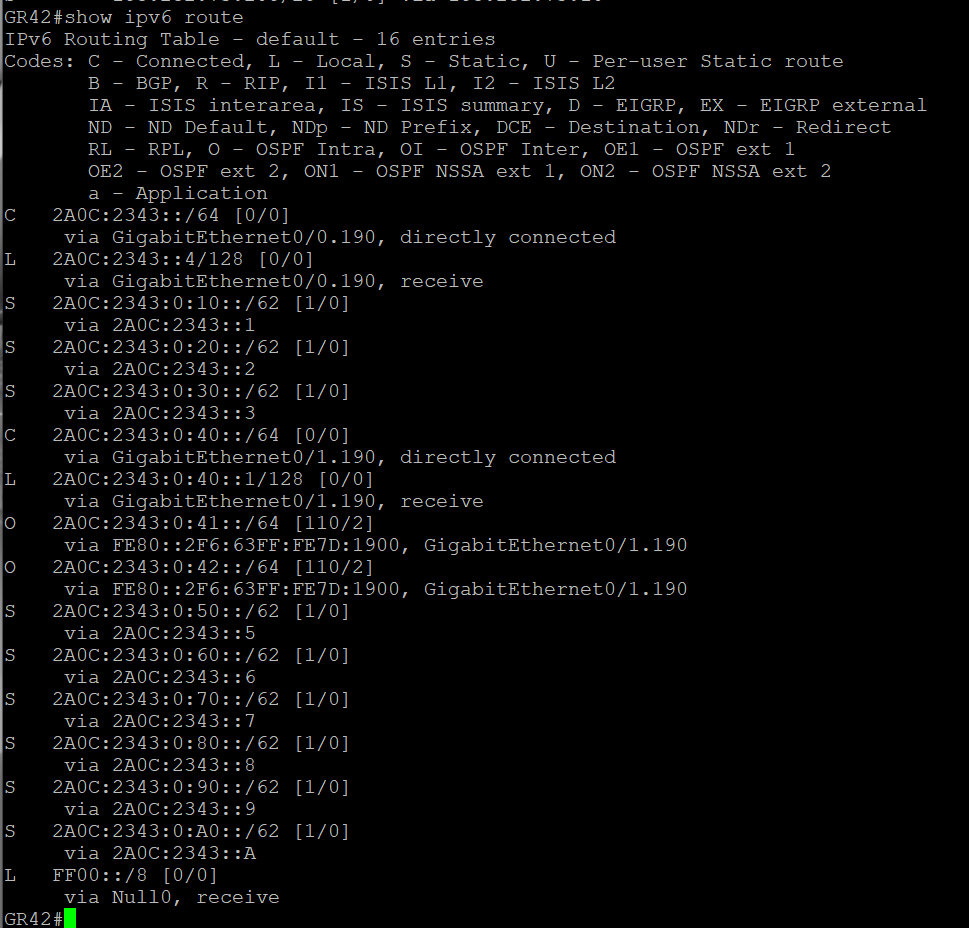
\includegraphics[width=\textwidth]{Arbeitsergebnisse/gr42/gr42_show_ipv6_route.png}
    \caption{GR42 show route (IPv4)}
  \end{minipage}
\end{figure}

\end{document}